\documentclass[11pt, oneside]{article} 
\usepackage{geometry}
\geometry{letterpaper} 
\usepackage{graphicx}
	
\usepackage{amssymb}
\usepackage{amsmath}
\usepackage{parskip}
\usepackage{color}
\usepackage{hyperref}

\graphicspath{{/Users/telliott_admin/Dropbox/Tex/png/}}
% \begin{center} 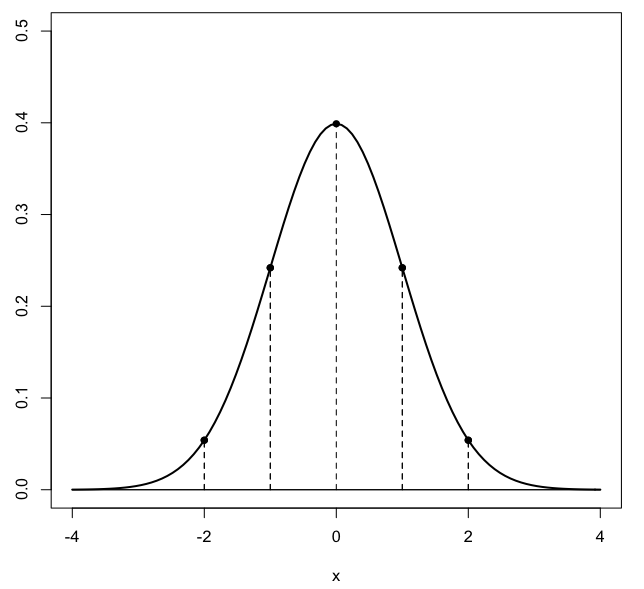
\includegraphics [scale=0.4] {gauss3.png} \end{center}

%break
\title{Newton square root}
\date{}

\begin{document}
\maketitle
\Large
Here is a method for finding roots of equations quickly, often called Newton's method, or the Newton-Raphson method.  As an example, here is a plot of the function
\[ f(x) = x^2 - 2 \]
\begin{center} 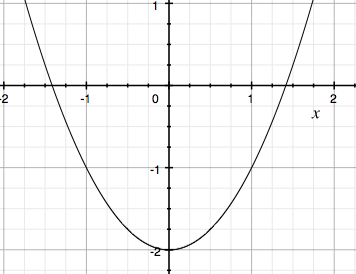
\includegraphics [scale=0.6] {sqrt2.png} \end{center}
which is equal to zero when $x = \pm \sqrt{2}$.  That is, we want the roots of the following equation
\[ x^2 - 2 = 0 \]
and more generally
\[ x^2 - N = 0 \]
to find the square root of some other number.  

Pick a point $g$ (for guess).  Then we need to construct the line tangent to the curve at that point, with slope $m=f'(g)$ and ask, where does this line intercept the $x$-axis?  

The slope is $\Delta y/ \Delta x$.

\[ \frac{f(g) - 0}{g - r} = f'(g) \]
with $r$ being the $x$-coordinate at the intercept.  Rearrange
\[ \frac{f(g)}{f'(g)} = g - r \]
\[ r = g - \frac{f(g)}{f'(g)} \]

\subsection*{square root problem}
For this particular problem, we have
\[ f(g) = g^2 - N \]
\[ f'(g) = 2g \]
\[ r = g - \frac{g^2 - N}{2g} = \frac{1}{2} (g + \frac{N}{g}) \]
In other words, $r$ is the average of $g$ and $N/g$.

Now set $g = r$ and repeat.

This can be encapsulated into the following algorithm:
\begin{itemize}
\item Make a guess $g$ and compute $N/g$
\item Average $g$ and $N/g$ to find a new guess
\item Repeat until satisfied
\end{itemize}

The algorithm converges rapidly for most problems.

\begin{verbatim}
2
1.5
1.4166666666666665
1.4142156862745097
1.4142135623746899
1.414213562373095
\end{verbatim}

\subsection*{notes}
It is worthwhile to try to make a good first guess.  If the method goes wrong (which it can, when equations have bumps or other issues), the problem can be fixed by making a better guess.

You can read more about the method here:

\url{http://www.math.ubc.ca/~anstee/math104/newtonmethod.pdf}

For the particular problem that we worked, finding the square root of $N$, the equation says
\[ g' = \frac{1}{2} (g + \frac{N}{g}) \]

find your next guess by averaging the current guess $g$ and $N/g$.  

This equation goes back at least as far as Heron of Alexandria (10-70 AD).



\end{document} 